\documentclass[12pt]{article}

\usepackage[]{listings}
\usepackage[]{graphicx}
\usepackage[dutch]{babel}
\usepackage[hidelinks]{hyperref}

\begin{document}

\title{The Basics of \LaTeX{}}
\author{Sander Hansen}
\date{\today}
\maketitle

\clearpage
\section{Inleiding}

\subsection{Grote rafelvis}
De grote rafelvis (Phycodurus eques), soms ook zeedraak genoemd, is een zeevis die verwant is aan de zeepaardjes. Het is de enige soort uit het geslacht Phycodurus. Hij komt in het zuiden en westen van Australie voor.

\begin{figure}[ht!]
\centering
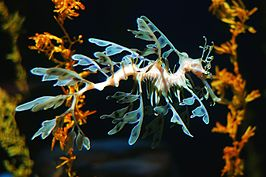
\includegraphics[]{zeedraak.jpg}
\caption{Zeedraak man}
\end{figure}

\subsection{Beschrijving}
De grote rafelvis leeft op met kelp begroeide riffen en in kelpwouden tussen de bladeren van deze wieren op een diepte tussen de 4 en 30 meter. Deze vis wordt niet groter dan 35 cm. De vis is uitstekend gecamoufleerd; het is het beste voorbeeld van camouflage waar zowel mensen als roofdieren de grootste moeite hebben om hem te vinden.
Net als bij andere soorten uit de familie van de zeenaalden en zeepaardjes geeft het vrouwtje als het met het mannetje paart haar eitjes aan het mannetje, die door hem bevrucht worden. Het mannetje draagt de eitjes onder zijn buik en staart in een broedbuidel tot ze uitkomen en weg gaan.
\\
Meer informatie over de zeedraken vindt u zeker niet op:
\href{http://student.uva.nl/inc/az}{Inleiding programmeren}

\section{Methode}

\begin{lstlisting}
public class HelloWorld {

	/*
	 * @param args
	 */
	 public static void main(String[] args) {
	 	// TODO Auto-generated method stub
	 	System.out.println("Hello world!");
	 }
}
\end{lstlisting}
\\

\section{Resultaten}

\section{Discussie}

Hello world!

\end{document}